\section{Data}
\label{sec:data}

For this work we utilise a sample of 68 revealing post-starburst spectral features drawn from the Sloan Digital Sky Survey SDSS-IV MaNGA (Mapping Nearby Galaxies at Apache Point Observatory) integral field spectroscopic survey. This sample, and a related control sample of approximately 680 normal galaxies (i.e. galaxies which do not exhibit PSB spectroscopic features),  were kindly provided by Chen et al. (2019, submitted).

\subsection{The SDSS-IV MaNGA survey}
\label{sec:MaNGA}
The data used in this work includes galaxy stellar velocity and gas velocity kinematic maps, spectral index maps and individual spectra drawn from the SDSS-IV MaNGA project. An overview of the MaNGA project is provided by \citet{2015ApJ...798....7B}. This paper describes key instrumentation features and outlines the observational strategy: MaNGA captures dithered observations with 17 fibre-bundle integral
field units (IFUs) varying in size from 19 fibres to 127 fibres and arranged in 3 to 7 hexagonal layers. Two dual-channel spectrographs provide
simultaneous wavelength coverage over the range 3600 to 10300 \AA\ at a spectral resolution of R$\sim$2000. MaNGA is an integral field spectroscopic survey (IFS) which provides spatially resolved images and maps of galaxy properties. The images and property maps can provide evidence of external kinematic influences such as close neighbour interaction, present merger activity and the signatures of past merger remnants.

IFU dithered data are processed in the MaNGA Data Reduction Pipeline (DRP) to produce calibrated spectra and rectified three-dimensional data cubes. The final data products (data cubes) of the DRP feed into the MaNGA data analysis pipeline (DAP) \citep{2016AJ....152...83L,2019arXiv190100856W} which, the purposes of this paper, provides:
\begin{itemize}
    \item Spatially stacked spectra
    \item Stellar kinematics (velocity, V, and velocity dispersion, $\sigma$)
    \item Nebular emission-line properties: fluxes, equivalent widths, and kinematics (V and $\sigma$)
    \item Spectral Indices: absorption-line (e.g.  H$\delta_A)$ and bandhead (e.g., D$_n$4000) measurements
\end{itemize}

Kinematic data is extracted from the MaNGA DAP output maps designated MAPS-SPX-GAU-MILESHC: where SPX denotes individual spaxel binning; GAU an algorithm for a  Gaussian fit to stellar spectra; and MILESHC is a reference to the MILES library \citep{2011A&A...532A..95F} of stellar spectrum templates. The DAP analysis algorithms are  described in the SDSS DR15 DAP documentation \citet{2019arXiv190100856W}. 2-D maps provide kinematic data: 

\begin{itemize}
    \item Projected stellar rotation velocity
    \item Stellar velocity dispersion
    \item Ionised gas rotational velocity
    \item Ionised gas velocity dispersion
\end{itemize}

Associated 3-D (2 spatial dimensions and 1 spectral wavelength dimension) data cubes, designated MAPS-VOR10-GAU-
MILESHC, provide spatial spectral series yielding the following spectral properties across the galaxy field-of-view:

\begin{itemize}
    \item D$_n$4000 spectral index as a measure of the strength of the 4000 \AA\ break
    \item H$\delta_A$ absorption spectral index
    \item Nebular emission line equivalent widths
\end{itemize}

The D$_n$4000 and H$\delta_A$ spectral indices are indicators of stellar age and therefore of star formation \citep{1997A&A...325.1025P}. 

The above datasets can be downloaded in the form of 3-D data cubes from the SDSS science archive server (SAS) or by using the Marvin web interface tool\footnote{\href{https://dr15.sdss.org/marvin/}{https://dr15.sdss.org/marvin/}} as described in \cite{2018arXiv181203833C}. SDSS and MaNGA data is released periodically in MaNGA Product Launches (MPL) each with an accompanying SDSS data release (DR) number. The current SDSS data release, DR15, is the third data release of the the fourth phase of the SDSS observational programme and includes all data from prior releases. In this project we use data cubes from MaNGA MPL-7, DR15 \citep{2019ApJS..240...23A}. The associated FITS-format galaxy data summary table output from DRP \texttt{drpAll} file is version 2.4.3 \citep{2016AJ....152...83L}. Some useful data fields from the \texttt{drpAll} data file used in this project are listed in Table \ref{tab:DRPall-table}.

\begin{table*}
\caption[MaNGA DRPALL fields used in the project]{SDSS-IV MaNGA DRPALL v2.4.3 data fields used in the project}
\label{tab:DRPall-table}
\begin{tabular}{|p{3.2cm}|p{1.2cm}||p{1cm}|p{10cm}|}
\hline
Name & Type & Unit & Description \\
\hline
PLATEIFU & char{[}100{]} &  & Plate+ifudesign name for this object (e.g. 7443-12701)\\
MANGAID & char{[}100{]} & & MaNGA ID for this object (e.g. 1-114145)\\
OBJRA & float64 & degrees & Right ascension of the science object in J2000\\
OBJDEC & float64 & degrees & Declination of the science object in J2000\\
NSA\_Z & float64 &  & Heliocentric redshift\\
NSA\_ZDIST & float64 &  & Distance estimate using peculiar velocity model of Willick et al. (1997); mulitply by c/Ho for Mpc\\
NSA\_ELPETRO\_MASS & float64 &  & Stellar mass from K-correction fit (use with caution) for elliptical Petrosian fluxes ($\Omega_m=0.3$, $\Omega_\Lambda=0.7$, $h=1$)\\
NSA\_ELPETRO\_BA & float64 &  & Axis ratio used for elliptical apertures (for this version, same as ba90)\\
NSA\_ELPETRO\_TH50\_R & float64 & arcsec & Elliptical Petrosian 50\% light radius in SDSS r-band\\
NSA\_SERSIC\_N & float64 &  & Se
rsic index from two-dimensional, single-component Sersic fit in r-band\\
\hline
\end{tabular}
\end{table*}

\subsection{Sample selection}
As noted in the introduction, post-starburst galaxies and regions of galaxies with PSB features can be identified from their spectra which typically exhibit the strong Balmer absorption lines of A-type stars. Additionally, weak or absent H$\alpha$ and/or [OII] emission lines indicate a quiescent state with little or no present star formation. 

The PSB and control galaxy samples provided by Chen et al. (2019, submitted, personal communication) were drawn from an analysis of 4633 galaxies made available from the earlier MPL-6\footnote{\href{}{https://sdss-marvin.readthedocs.io/en/stable/datamodel/mpl6.html}} (MaNGA Product Launch 6). The objective being to identify galaxies possessing PSB regions in which star formation was rapidly quenched in the past 1 to 2 Gyr leaving no spectral evidence of stars younger than A-type.  Chen et al. (2019, submitted) adopted the following sample selection criteria:
\begin{itemize}
    \item Spaxels with signal-to-noise S/N > 10 per pixel
    \item Strong H$\delta_A$ absorption line > 3\AA 
    \item A strong 4000 \AA\ break 
    \item Weak H$\alpha$ equivalent width W(H$\alpha$) < 10\AA
    \item and $\log{W(H\alpha)} < 0.23\times{H\delta_A}-0.46$
\end{itemize}
The H$\delta_A$ absorption spectral index is the equivalent width of H$\delta$ 4102\AA\ line as described by \citet{1994ApJS...94..687W}. In addition to the above criteria, for a region of a galaxy to be classed as post-starburst at least 6 contiguous spaxels from the DAP analysis are required. 

Chen et al. (2019, submitted) identified a total of 360 galaxies possessing PSB spaxel regions meeting the above selection criteria and categorised them into 3 PSB types: those with central PSB regions (CPSBs); those with off-centre ring-like, or partial ring-like PSB features (RPSBs) and those with irregular regions of PSB spaxels in the outskirts (irregular PSBs or IPSBs). The PSB selection from Chen et al. (2019) yielded a total of 31 CPSBs and 37 RPSBs. Useful properties from the MaNGA \texttt{drpAll} file for the selected PSBs are listed in appendix \ref{sec:lists-of-psbs}, Tables \ref{tab:my-CPSBs} and \ref{tab:my-RPSBs} respectively. We will use the data in these tables frequently throughout this report to investigate the distribution of various parameters between the PSB groups and their control samples.

The colour-mass distribution of the CPSB and RPSB samples is shown in Figure \ref{fig:Colour-Mass-PSBs}. The contour plot represents the complete population of MaNGA DR15 galaxies plotted as the NSA (NASA Sloan atlas) colour index NUV-i values versus galaxy stellar mass obtained from the NSA data field  NSA\_ELPETRO\_LOGMASS. Our PSB samples are superimposed on the DR15 full population density contour plot. We note that the population of CPSBs generally lie redward of the RPSBs as shown in the colour-mass diagram of Figure \ref{fig:Colour-Mass-PSBs}. The mass distributions of the two PSB populations are similar, however.

\begin{figure}
    \centering
    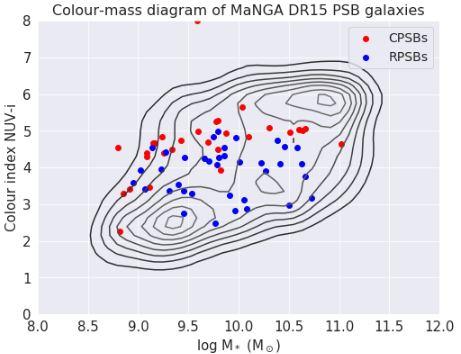
\includegraphics[width=\columnwidth]{images/CMDs/CMD-CPSB+RPSB-15.png}
    \caption[Colour-mass distribution of PSBs]{The sample of PSB galaxies is shown distributed over the complete DR15 population density contour plot as shown in Figure \ref{fig:CMD-mass-1}. CPSBs are represented by red dots and RPSBs as blue dots.}
    \label{fig:Colour-Mass-PSBs}
\end{figure}

\subsection{Control galaxies}
\label{sec:controls}
A control sample set of regular galaxies not exhibiting PSB features was also selected by Chen et al. (2019). The purpose of the control sample is to provide a reference set of properties for comparison with the PSB data with a view to identifying typical progenitors which have not (yet) experienced a major merger. For each PSB group (CPSBs and RPSBs), a set of 10 non-PSB galaxies were selected but having similar stellar mass and global D$_n$4000 spectral indices. We have used this control galaxy sample in this work to highlight the differences of the properties of PSBs compared to regular (non-PSB) galaxies.

Colour-mass diagrams of the two PSB groups with subsets of their control group samples are presented in Figure \ref{fig:Colour-Mass-PSBs-controls}. The colour-mass distribution of each of the PSB groups, CPSBs and RPSBs, is generally similar to that of their respective control groups. This confirms that the general objectives of control selection was achieved.

\begin{figure*}
    \centering
    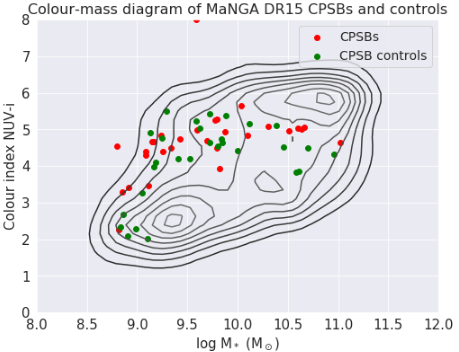
\includegraphics[width=\columnwidth]{images/CMDs/CMD-CPSBs+Controls-15.png}
    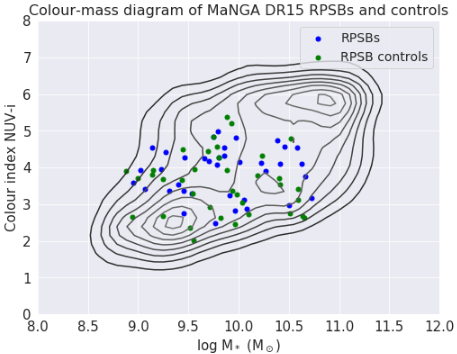
\includegraphics[width=\columnwidth]{images/CMDs/CMD-RPSBs+Controls-15.png}
    \caption[Colour-mass distribution of PSBs and controls]{The contents are similar to Figure \ref{fig:Colour-Mass-PSBs}. The colour-mass distribution of PSBs and their control galaxies has been superimposed on the contour plot of the complete DR15 population. The left panel shows the distribution of the CPSB sample (red dots) with their control galaxies (green dots), in the right panel the RPSB sample (blue dots) with their corresponding controls (again with green dots).}
    \label{fig:Colour-Mass-PSBs-controls}
\end{figure*}

\subsection{PSB spectra}
The central spaxel spectrum of the CPSB galaxy 8623-9102 is shown in Figure \ref{fig:CPSB-8623-9102-spec}. Spectral features include a Balmer break and strong hydrogen absorption lines in the wavelength region 3500 to 4500 \AA. In the same figure we compare the spectral features of the PSB to those of the regular (non-PSB) control galaxy 8990-3703 which has a similar mass to 8623-9102. In contrast, the spectrum of the control galaxy displays the strong hydrogen emission line feature of a star forming galaxy.

\begin{figure*}
    \centering
    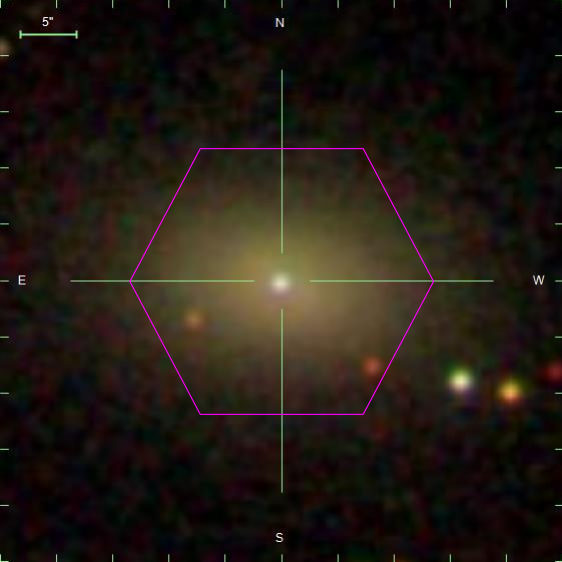
\includegraphics[width=0.22\textwidth]{images/Cutouts/CPSB-8623-9102-IM.png}
    \hfill
    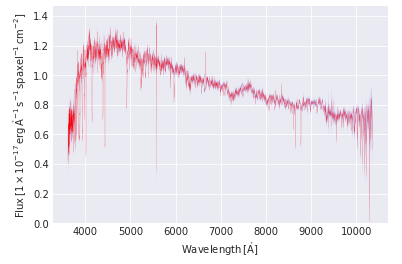
\includegraphics[width=0.38\textwidth]{images/Spectra/CPSB-8623-9102.png}
    \hfill
    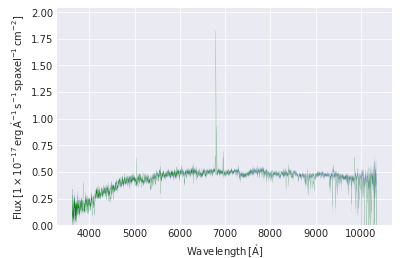
\includegraphics[width=0.38\textwidth]{images/Spectra/CPSB-CTRL-8990-3703-spec.png}
    \caption[Central spaxel spectrum of CPSB 8623-9102]{Left: SDSS 3-colour image of central-type PSB 8623-9102. 
    Centre: The spectrum of the central spaxel of CPSB  8623-9102. Note the Balmer break feature and strong hydrogen absorption lines in the wavelength region 3500 to 4500 \AA.
    Right: For comparison with the centre panel, the central spaxel spectrum of control galaxy 8990-3703 shows a strong H$\alpha$ emission line indicating the presence of ongoing star formation.}
    \label{fig:CPSB-8623-9102-spec}
\end{figure*}


The spectrum obtained from the central spaxel of a ring-type RPSB galaxy is shown in Figure \ref{fig:RPSB-8323-6103-spec}. The central spectrum (spaxel coordinates [27,27]) shows strong H$\alpha$ emission consistent with the presence of an ample gas supply for continuing star formation. However, moving away from the central spaxel, in the direction towards the upper right of the IFU hexagonal frame, the spectrum at spaxel coordinates [34,32] exhibits the characteristics of a post-starburst region. The spectrum in this region reveals weak emission lines and strong Balmer absorption lines typical of the stellar atmospheres of A-type stars. These features are consistent with the presence of a ring-type PSB feature at this location.

\begin{figure*}
    \centering
    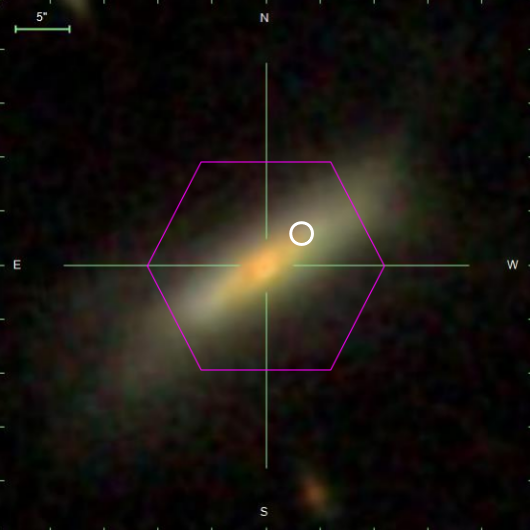
\includegraphics[width=0.24\textwidth]{images/Cutouts/RPSB-8323-6103-CIRCLED.png}
    \hfill
    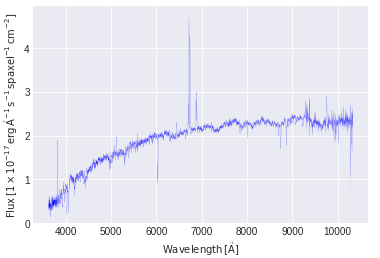
\includegraphics[width=0.35\textwidth]{images/Spectra/RPSB-8323-6103-27-27.png}
    \hfill
    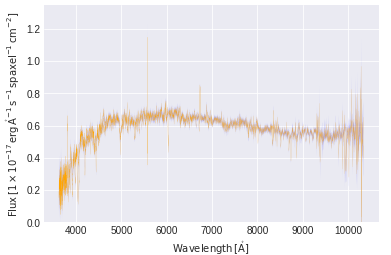
\includegraphics[width=0.35\textwidth]{images/Spectra/RPSB-8323-6103-34-32.png}
    \caption[Image and central and offset spectra of the RPSB 8323-6103]{The SDSS gri image, central and offset spectra of the RPSB 8323-6103. Left: SDSS 3-colour image. 
    Centre: the spectrum of the central region of the ring-type PSB 8323-6103 at spaxel coordinates [27, 27] revealing strong H$\alpha$ emission. 
    Right: the spectrum of ring-type PSB 8323-6103 at offset spaxel coordinates [34, 32].  The spectra of spaxels in this region exhibit typical post-starburst features of weak emission lines and strong Balmer absorption lines. This location is above and to the right of centre, as indicated in the left panel gri image by the white circle.}
    \label{fig:RPSB-8323-6103-spec}
\end{figure*}

\subsection{Velocity maps}
Our kinematic studies employ stellar and gas velocity maps obtained from MaNGA data  cubes. Examples of MaNGA stellar velocity and gas velocity maps for the CPSB 8313-6101 are given in Figure \ref{fig:CPSB-8313-6101-VMAPS}. In our kinematic analysis we are looking for irregularities in the velocity fields, such as departures from uniform circular motion, misalignment of the rotational axes of stellar and gas velocity fields,  and non-linear radial variation, any of which may provide evidence of past merger activity.

\begin{figure*}
    \centering
    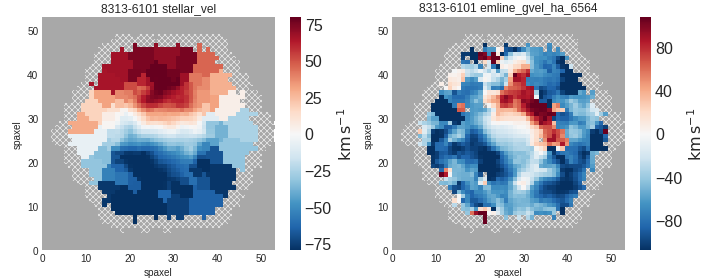
\includegraphics[width=0.9\textwidth]{images/VelocityMaps/CPSB-8313-6101-VMAPS.png}
    \caption[MaNGA velocity maps for CPSB 8313-6101]{MaNGA velocity maps for CPSB 8313-6101: stellar velocity (left) and H$\alpha$ gas velocity (right).}
    \label{fig:CPSB-8313-6101-VMAPS}
\end{figure*}



